\section{Microfrontends}

\begin{frame}
\frametitle{Microfrontends}
	\begin{figure}
		\centering
		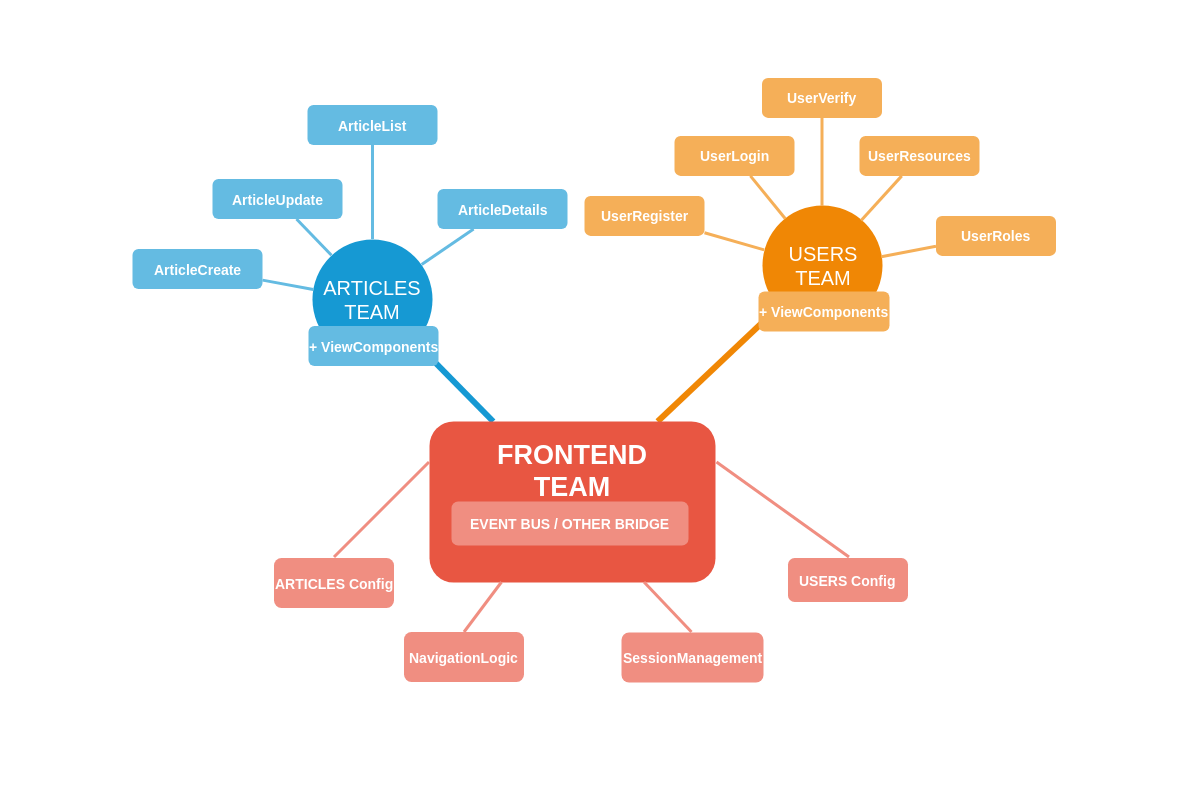
\includegraphics[width=0.9\linewidth]{pictures/microfrontends-knowledge.png}		
		\label{fig:microservices}
	\end{figure}
\end{frame}

\begin{frame}
\frametitle{Webcomponents}
Additional HTML tags defined in java script files, which can be shared between a lot of pages.
\begin{figure}
	\centering
	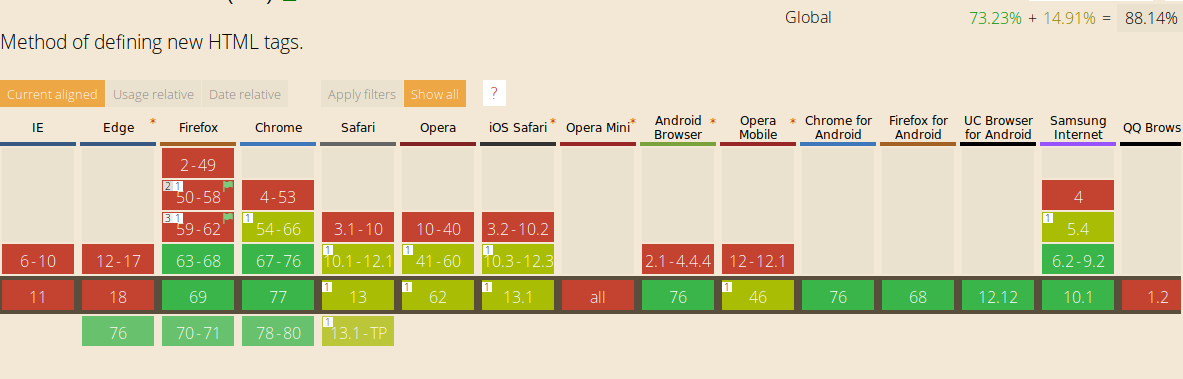
\includegraphics[width=0.9\linewidth]{pictures/webcomponents-support.png}		
	\label{fig:microservices}
\end{figure}
\end{frame}

\begin{frame}
\frametitle{Comparison}
\begin{figure}
	\centering
	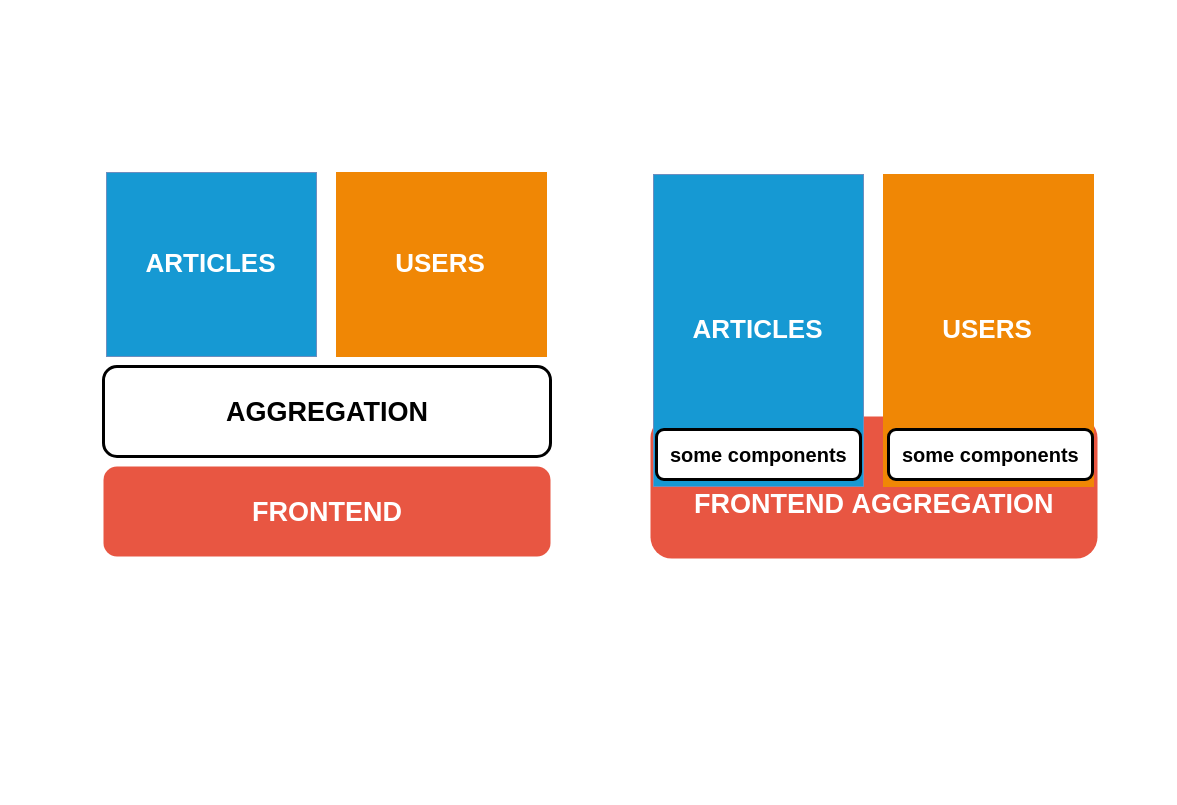
\includegraphics[width=0.9\linewidth]{pictures/microfrontends-vs-microservices.png}		
	\label{fig:vs}
\end{figure}
\end{frame}